\documentclass[border=5pt]{standalone}
\usepackage{tikz}
\usepackage{amsmath}
\usetikzlibrary{positioning, arrows.meta, calc, fit, backgrounds}

% --- Color Scheme (Purple-Blue) ---
\definecolor{bgPrimary}{HTML}{E8DAEF}
\definecolor{bgSecondary}{HTML}{D4E6F1}
\definecolor{bgAccent}{HTML}{D2B4DE}
\definecolor{bgInput}{HTML}{F4ECF7}
\definecolor{borderPrimary}{HTML}{AF7AC5}
\definecolor{borderAccent}{HTML}{7D3C98}
\definecolor{arrowColor}{HTML}{6C3483}
\definecolor{textMain}{HTML}{2C2C54}
\definecolor{textLight}{HTML}{7F8FA6}
\definecolor{bgHighlight}{HTML}{FDEBD0}

% --- Styles ---
\tikzset{
  module/.style={
    draw=borderPrimary, fill=bgPrimary, rounded corners=4pt,
    minimum width=2.6cm, minimum height=1.2cm,
    font=\sffamily\small, text=textMain, line width=0.6pt, align=center,
  },
  novelmodule/.style={
    draw=borderAccent, fill=bgAccent, rounded corners=4pt,
    minimum width=2.6cm, minimum height=1.2cm,
    font=\sffamily\small\bfseries, text=textMain, line width=1.0pt, align=center,
  },
  iobox/.style={
    draw=borderPrimary, fill=bgInput, rounded corners=3pt,
    minimum width=2.0cm, minimum height=1.0cm,
    font=\sffamily\small, text=textMain, line width=0.5pt, align=center,
  },
  plusnode/.style={
    circle, draw=borderPrimary, fill=bgSecondary,
    inner sep=0pt, minimum size=16pt,
    font=\sffamily\scriptsize\bfseries, text=textMain, line width=0.5pt,
  },
  groupbox/.style={
    draw=borderPrimary, fill=bgSecondary, fill opacity=0.2,
    rounded corners=6pt, inner sep=8pt, line width=0.5pt, dashed,
  },
  stdarrow/.style={
    -{Stealth[length=5pt, width=4pt]}, line width=0.6pt, color=arrowColor,
  },
}

\begin{document}
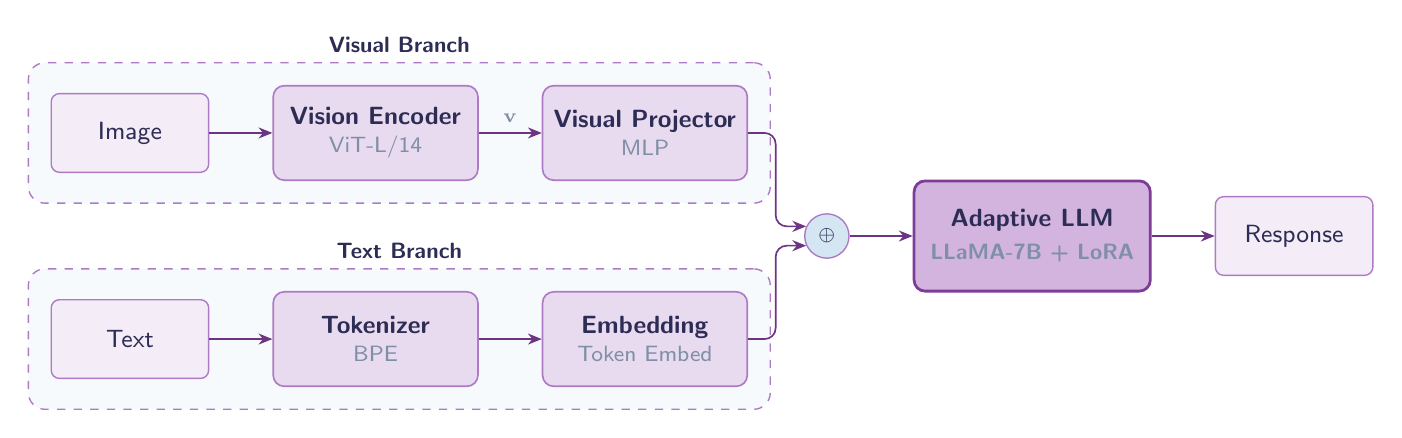
\begin{tikzpicture}

  % === Image Branch (top row) ===
  \node[iobox] (imgIn) {Image};
  \node[module, right=0.8cm of imgIn] (vit) {\textbf{Vision Encoder}\\[-1pt]{\footnotesize\color{textLight}ViT-L/14}};
  \node[module, right=0.8cm of vit] (proj) {\textbf{Visual Projector}\\[-1pt]{\footnotesize\color{textLight}MLP}};

  % === Text Branch (bottom row) — align under image branch ===
  \node[iobox, below=1.6cm of imgIn] (txtIn) {Text};
  \node[module, right=0.8cm of txtIn] (tok) {\textbf{Tokenizer}\\[-1pt]{\footnotesize\color{textLight}BPE}};
  \node[module, right=0.8cm of tok] (embed) {\textbf{Embedding}\\[-1pt]{\footnotesize\color{textLight}Token Embed}};

  % === Merge node — placed to the right of proj (furthest-right branch),
  %     vertically centered between the two branches ===
  \coordinate (midY) at ($(imgIn.center)!0.5!(txtIn.center)$);
  \coordinate (catTemp) at ($(proj.east)+(1.0cm,0)$);
  \node[plusnode] (cat) at (catTemp |- midY) {$\oplus$};

  % === LLM (novel) ===
  \node[novelmodule, right=0.8cm of cat, minimum width=3.0cm, minimum height=1.4cm]
    (llm) {\textbf{Adaptive LLM}\\[1pt]{\footnotesize\color{textLight}LLaMA-7B + LoRA}};

  % === Output ===
  \node[iobox, right=0.8cm of llm] (output) {Response};

  % === Arrows: image branch — orthogonal routing into cat from above-left ===
  \draw[stdarrow] (imgIn) -- (vit);
  \draw[stdarrow] (vit) -- node[above, font=\sffamily\scriptsize, text=textLight] {$\mathbf{v}$} (proj);
  \draw[stdarrow, rounded corners=4pt] (proj.east) -- ++(0.35cm, 0) |- (cat.155);

  % === Arrows: text branch — orthogonal routing into cat from below-left ===
  \draw[stdarrow] (txtIn) -- (tok);
  \draw[stdarrow] (tok) -- (embed);
  \draw[stdarrow, rounded corners=4pt] (embed.east) -- ++(0.35cm, 0) |- (cat.205);

  % === Arrows: merge to output ===
  \draw[stdarrow] (cat) -- (llm);
  \draw[stdarrow] (llm) -- (output);

  % === Group boxes ===
  \begin{scope}[on background layer]
    \node[groupbox, fit=(imgIn)(vit)(proj),
      label={[font=\sffamily\footnotesize\bfseries, text=textMain]above:Visual Branch}] {};
    \node[groupbox, fit=(txtIn)(tok)(embed),
      label={[font=\sffamily\footnotesize\bfseries, text=textMain]above:Text Branch}] {};
  \end{scope}

\end{tikzpicture}
\end{document}
